\section{An error budget for the distance scale}
\label{sec:budget}

Every recovered expansion rate in this paper is low, on both families of mocks,
and the offset does not average down with the number of events. This section
reports what it is made of, on the matched single-tracer mock
(\S\ref{sec:methods:mocks}). The budget closes: it decomposes into two further
respects in which the mock, as generated, was not a draw from the assumed model
--- each identified, measured, and repaired --- and an estimator overhead that
is measured against an exact evaluation of the likelihood
(\S\ref{sec:budget:oracle}, Figure~\ref{fig:waterfall}).

\subsection{The offset survives a matched generative process}
\label{sec:budget:closure}

Splitting the \CloNobs-event sample into \CloBlockN\ disjoint blocks --- whose
scatter measures gravitational-wave realisation noise while a common offset is
systematic, since the host catalog and injection campaign are shared and do not
average down --- gives a mean expansion rate of \CloBlockMeanHzero~\kmsmpc, i.e.\
an offset of \CloBlockOffset$\pm$\CloBlockSem~\kmsmpc, or
\CloBlockSig$\sigma$. Reseeding the catalog, the events and the posterior
samples together over \CloSeedN\ independent realisations, so that the result is
marginalised over catalog realisations rather than conditional on one, gives
\CloSeedOffset$\pm$\CloSeedSem~\kmsmpc, \CloSeedSig$\sigma$. The offset is real
and it is not a property of one catalog.

It is also not carried by a minority of pathological events. Dividing the sample
into \CloLocNBlocks\ disjoint blocks of \CloLocBlockSize\ events, the per-event
log-likelihood pull has mean \CloLocPullMean\ with a median absolute deviation of
\CloLocPullMad\ and \CloLocOutliers\ outlying blocks: the pull is spread evenly
across the sample, which is what a convention or normalisation error looks like
rather than a few bad events.

Several candidate explanations were measured and eliminated. Matching the host
rate index to the mock's own host draw moves \Hz\ by \CloLeverGamma~\kmsmpc.
Truncating the catalog to a third or a seventh of its hosts --- which moves the
redshift boundary a long way while leaving every host the events can use ---
changes the result by at most $\CloLeverDepthMax$~\kmsmpc, because at $K=1$ the
survey-global normalisation cancels between the per-event terms and the selection
term. Coarsening the sky pixelisation moves it by \CloLeverNside~\kmsmpc. And
the selection integral itself is right: its logarithmic derivative with respect
to \Hz\ at the truth is \CloDecompDlnmu, matching the analytic expectation for a
distance-limited survey. What remains is the per-event term: at the truth the
per-event sum alone peaks at \CloDecompNum~\kmsmpc, \CloDecompNumOff\ high, and
the selection term shifts the total by \CloDecompShift\ to
\CloDecompTotal~\kmsmpc.

\subsection{The offset scales with the measurement noise}
\label{sec:budget:noise}

Holding the catalog, the events' true parameters and the injection campaign fixed
and varying only the fractional distance uncertainty gives a clean scaling
(Figure~\ref{fig:budget}a). With posterior samples drawn about the true
parameters the offset is \CloTruthSigOneOff~\kmsmpc\ at
$\sigma_{d_L} = \CloSigLo$, \CloTruthSigThreeOff\ at $\CloSigMid$ and
\CloTruthSigTenOff\ at $\sigma_{d_L} = \CloSigHi$; with samples drawn about a
noisy observation --- the construction a real parameter-estimation run produces
--- it is \CloCorrSigOneOff, \CloCorrSigThreeOff\ and \CloCorrSigTenOff. Both
series vanish as the noise vanishes and grow roughly quadratically in it, which
says the offset lives in the measurement-noise channel rather than in the
noiseless likelihood. Correcting the posterior construction closes the
zero-noise limit essentially exactly but leaves the offset at realistic noise
almost unchanged, so it isolates the channel and not the mechanism: a $\sigma^2$
scaling is consistent with any defect that scales with the noise level. The
defects identified in \S\ref{sec:budget:detection} and
\S\ref{sec:budget:oracle} both do.

\subsection{Half of it is a detection rule that acted on the wrong data}
\label{sec:budget:detection}

The mechanism we can identify is a mismatch between what decided detection and
what the likelihood conditions on. If a source is kept or discarded on the basis
of a latent variable that does not appear in the data --- a random projection
factor entering the signal-to-noise, say, drawn independently of the noise
realisation the parameter estimation conditions on --- then the correct
detected-set likelihood carries an extra factor of $P({\rm det}|\theta)$
\emph{inside} each event's integral,
\begin{equation}
  p(\{d_i\} \,|\, \Lambda, {\rm det}) =
  \frac{\prod_i \int \dd\theta\, p(d_i|\theta)\, p(\theta|\Lambda)\,
        P({\rm det}|\theta)}{\mu(\Lambda)^{\Nobs}},
  \label{eq:detcoupling}
\end{equation}
whereas every population code --- correctly, for a real detector --- evaluates
$\prod_i [\int p(d_i|\theta) p(\theta|\Lambda) \dd\theta] / \mu^{\Nobs}$, which
is exact when detection is a deterministic function of the data so that the
indicator drops out. The inference is not wrong; the mock is not a draw from it.

We measured the size of that effect with a paired experiment over
\AbCtrlN\ realisations in which the two arms share the host catalog, the event
seed and every ancillary uncertainty model, so their difference is the detection
rule alone (Figure~\ref{fig:budget}b, Table~\ref{tab:budget}). The control arm,
with detection decided by the latent projection factor, gives an offset of
\AbCtrlMean$\pm$\AbCtrlSem~\kmsmpc\ (\AbCtrlSig$\sigma$), reproducing the
independent \CloSeedN-realisation measurement of
\AbBaselineMean$\pm$\AbBaselineSem\ and licensing the comparison. Moving
detection onto a single observed measurement per source, which is then also what
the posterior conditions on, gives \AbObsMean$\pm$\AbObsSem~\kmsmpc\
(\AbObsSig$\sigma$). The paired difference is
\AbDiffMean$\pm$\AbDiffSem~\kmsmpc, \AbDiffSig$\sigma$ from zero, or
\AbFracRemoved\% of the control offset. The projection latent cannot simply be
retained in the corrected arm --- that would leave detection depending on a
variable absent from the data, which is a different mismatch rather than a fix
--- so the reference signal-to-noise was recalibrated, to \AbObsSnrRef, to
reproduce the control's detected fraction; the two arms' event populations then
agree to a few per cent in median redshift, and each arm carries its own
injection campaign of \AbObsInjNdraw\ million proposals.

After this correction the campaign offset is
\CloResidual$\pm$\CloResidualSem~\kmsmpc, still \CloResidualSig$\sigma$ from
zero. The next subsection splits it.

\subsection{The rest is the mock again, plus the estimator's overhead}
\label{sec:budget:oracle}

The generative process of this mock is simple enough that the likelihood it
implies can be evaluated \emph{exactly} --- the host marginal as a discrete
sum over the catalog, the mass integrals and the selection function by
deterministic quadrature, no Monte Carlo anywhere --- and the exact evaluation
splits the residual cleanly. Over the \OrcN\ realisations of the campaign, the
exact likelihood itself recovers the expansion rate low, by
\OrcExactOff$\pm$\OrcExactSem~\kmsmpc\ (\OrcExactSig$\sigma$). Equivalently,
the score identity that any detected-set likelihood must satisfy at the truth
fails: the mean per-event score falls short of the
$\dd\ln\mu/\dd\Hz = \OrcScoreDemand$ the identity demands by
\OrcScoreDef$\pm$\OrcScoreDefSem\ per event per \kmsmpc. Most of the residual
is therefore not the inference at all: it is a third respect in which the mock
was not a draw from the model, of the same family as the last two. Each
event's sky-localisation width was drawn as a deterministic function of its
\emph{latent true} masses and distance
($\sigma_{\rm ang} \propto d_L / \mathcal{M}_c^{5/6}$, the scaling of an
optimal signal-to-noise) and then handed to the parameter estimation as known
metadata. The width is thereby itself a distance-sensitive --- hence
\Hz-sensitive --- observable, and a fixed-width sky posterior cannot represent
it: events whose true host received a large sky residual systematically
down-weight that host, and the omission has non-zero mean score at the truth.
The proof is a paired generator experiment under the exact likelihood: fresh
event sets drawn with the recipe as-is give
\OrcBootAsisOff$\pm$\OrcBootAsisSem~\kmsmpc, and deriving the width from the
\emph{observed} masses and distance --- measuring first, then localising ---
gives \OrcBootFixOff$\pm$\OrcBootFixSem\ and restores the score identity.
That is closure.

The three defects state one requirement three ways: for a dark-siren mock to
be a draw from the model, every quantity the likelihood conditions on as fixed
metadata --- the posterior samples' centring, the detection decision, the
per-event uncertainty widths --- must be a function of the observed data, not
of the latent true parameters. Violations do not announce themselves; each of
the three produced a smooth, stable, noise-scaled offset of the same sign that
survived every conventional robustness test in
\S\ref{sec:budget:closure}--\ref{sec:budget:noise}. The score identity at the
truth, evaluated under an exact likelihood, is the diagnostic that finds them.

What genuinely belongs to the inference is the paired difference between the
production estimator and the exact likelihood on the same events:
\OrcPairedOff$\pm$\OrcPairedSem~\kmsmpc\ (\OrcPairedSig$\sigma$). Its budget
is itself measured (Figure~\ref{fig:waterfall}): the $1/\Neff$
selection-variance correction \citep{Farr2019} tilts the posterior by
\OrcFarr~\kmsmpc\ because \Neff\ rises with \Hz; sky pixelation contributes
\OrcPix$\pm$\OrcPixSem, the sample-basis Jacobian \OrcJac, the fixed-width
mass kernels \OrcPeWidth\ and the catalog kernel smoothing \OrcKde. On top of
these systematic terms the selection estimator carries a zero-mean noise of
\OrcMuNoiseSd~\kmsmpc\ per realisation (mean \OrcMuNoiseMean) from the
interaction of the shared injection set with each catalog's kernel support ---
injections drift in and out of contact with individual host kernels as \Hz\
rescales the distance--redshift map --- which is invisible to any single-catalog
analysis and is part of why the per-realisation intervals of
\S\ref{sec:budget:samplevariance} are too narrow. The practical statement for
selection budgeting: an effective-sample-size floor guards the mean of the
selection estimate but not this \Hz-dependent wander, which should be budgeted
through the estimator's variance as a function of the scanned parameter rather
than at a single point.

The regenerated campaign confirms the attribution end to end on full
production mocks. Rebuilding all \CloFixN\ realisations with the repaired
generator and rerunning the production estimator moves the offset from
\CloResidual$\pm$\CloResidualSem\ to \CloFixMean$\pm$\CloFixSem~\kmsmpc, a
paired per-realisation improvement of \CloFixDiff$\pm$\CloFixDiffSem; what
remains agrees with the exact-likelihood attribution realisation by
realisation (repaired campaign minus exact likelihood on the original events:
\CloFixVsOracle$\pm$\CloFixVsOracleSem) and is the estimator overhead of the
previous paragraph, not the mock.

\begin{figure}
\centering
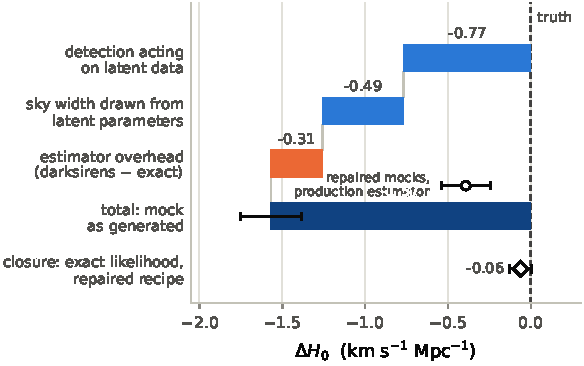
\includegraphics[width=\columnwidth]{figures/fig_closure_waterfall.pdf}
\caption{The distance-scale budget closes. From the campaign offset of the
mock as generated, the two generator defects --- detection acting on latent
data (\S\ref{sec:budget:detection}) and a sky-localisation width derived from
latent parameters (\S\ref{sec:budget:oracle}) --- account for their measured
shares, leaving the estimator-minus-exact-likelihood overhead, whose own
budget is the Farr $1/\Neff$ term plus zero-mean selection-Monte-Carlo noise.
The open circle is the regenerated campaign --- the production estimator on
repaired-generator mocks --- which lands on the overhead, as the attribution
predicts; the open diamond is the closure endpoint, the exact likelihood on
events drawn with the repaired recipe.
\label{fig:waterfall}}
\end{figure}

\begin{figure*}
\centering
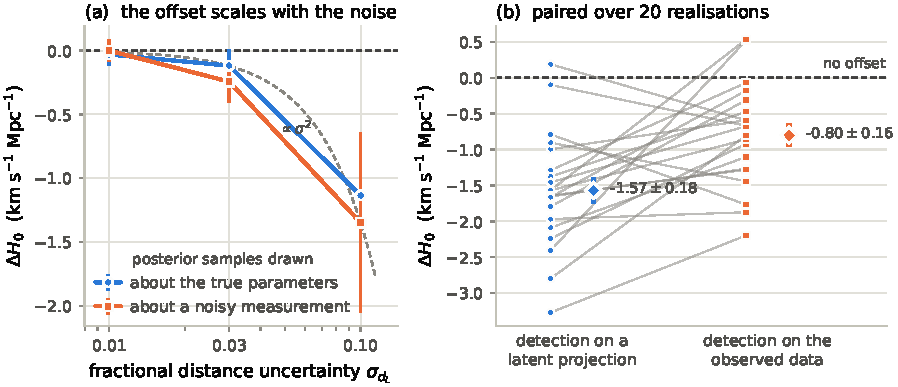
\includegraphics[width=\textwidth]{figures/fig_bias_budget.pdf}
\caption{Error budget of the distance scale on the matched single-tracer mock.
\emph{(a)} the offset against the fractional distance uncertainty, for posterior
samples drawn about the true parameters and about a noisy observation, with a
quadratic reference anchored on the corrected arm; both series vanish with the
noise. \emph{(b)} the paired detection-rule experiment over \AbCtrlN\
realisations. Thin lines join the two arms of the same realisation; diamonds are
the arm means with their standard errors. Moving detection onto the data the
posterior conditions on removes \AbFracRemoved\% of the offset and leaves
\CloResidualAbs$\pm$\CloResidualSem~\kmsmpc, which
\S\ref{sec:budget:oracle} splits between a third generator defect and the
estimator's overhead.
\label{fig:budget}}
\end{figure*}

\begin{deluxetable*}{lccc}
\tablecaption{Error budget of the distance scale on the matched single-tracer mock. The first row is the offset the mock as generated produces; the second is the paired difference between two arms that differ only in the detection rule; the third is the offset of the exact likelihood itself, which isolates the latent sky-width defect; the fourth is the paired difference between the production estimator and the exact likelihood on the same events. The last row is the closure endpoint: the exact likelihood on events drawn with the repaired recipe. \label{tab:budget}}
\tablehead{\colhead{} & \colhead{$N_{\rm real}$} & \colhead{$\Delta H_0$ (\kmsmpc)} & \colhead{$\sigma$}}
\startdata
offset as generated & 20 & $-1.570\pm0.184$ & 8.5 \\
detection acting on latent data & 20 & $+0.768\pm0.226$ & 3.4 \\
sky width drawn from latent parameters & 20 & $-0.489\pm0.077$ & 6.4 \\
estimator overhead (vs.\ exact likelihood) & 20 & $-0.312\pm0.125$ & 2.5 \\
\hline
closure: exact likelihood, repaired recipe & 20 & $-0.062\pm0.066$ & 0.9 \\
\enddata
\tablecomments{Independent of the offset, the host-catalog realisation contributes $0.97$~\kmsmpc\ of scatter per 1000-event realisation, which the per-realisation intervals do not contain: the realised scatter is 2.2$\times$ the quoted 68\% half-width.}
\end{deluxetable*}


\subsection{The host catalog is a random realisation, and it matters}
\label{sec:budget:samplevariance}

Independently of any offset, the \CloSeedN-realisation run measures something
that dark-siren error budgets do not usually contain. The realisation-to-real\-i\-sa\-tion
standard deviation of the recovered expansion rate is
\CloSeedScatter~\kmsmpc, against a mean quoted 68\% half-width of
\CloSeedMeanHw~\kmsmpc\ (Figure~\ref{fig:samplevar}). The credible intervals are
therefore too narrow by a factor of \CloSeedUnderFactor, and
quadrature-subtracting them from the realised scatter leaves
\CloCatalogVariance~\kmsmpc\ of scatter per \CloNobs-event sample attributable
to the host catalog realisation itself, at this catalog density.

The reason is structural rather than incidental. A credible interval computed
with one catalog is conditional on that catalog: it propagates the
gravitational-wave measurement uncertainty and the selection estimate, but the
catalog enters as a fixed object, so the fact that a different realisation of the
same density field would have placed hosts differently is nowhere in it. At this
density the missing term is comparable in size to the offset of
\S\ref{sec:budget:detection}, so it is not a refinement. Any dark-siren analysis
that quotes an interval at fixed catalog --- which is to say, any analysis using
a single real catalog --- is missing a term of this character, and its size has
to be established by realisation rather than assumed small.

\begin{figure*}
\centering
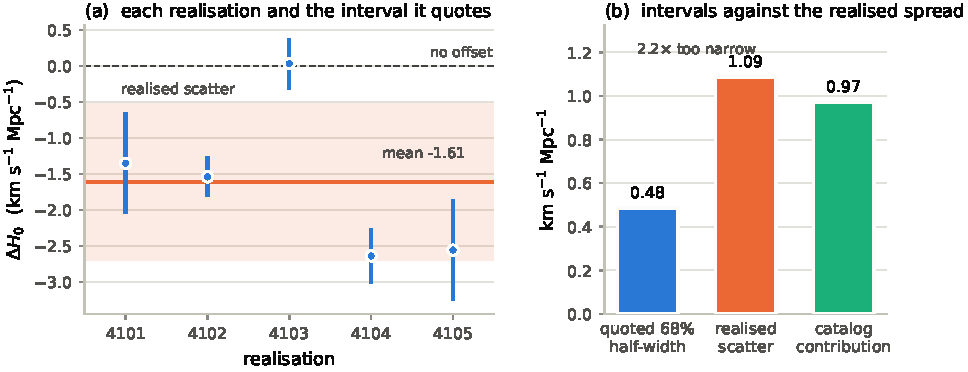
\includegraphics[width=\textwidth]{figures/fig_sample_variance.pdf}
\caption{Host-catalog sample variance. \emph{(a)} \CloSeedN\ realisations in
which the catalog, the events and the posterior samples are reseeded together,
each with the 68\% interval it quotes; the band is the realised scatter about the
mean. \emph{(b)} the same statement as a budget: the realised scatter exceeds the
quoted half-width by a factor of \CloSeedUnderFactor, and the excess in
quadrature, \CloCatalogVariance~\kmsmpc, is the catalog realisation's own
contribution.
\label{fig:samplevar}}
\end{figure*}
